\documentclass[12pt]{article}
\usepackage{amsmath,amssymb,bookmark,graphicx,parskip,custom}
\usepackage[margin=.8in]{geometry}
\allowdisplaybreaks
\hypersetup{colorlinks,
    citecolor=black,
    filecolor=black,
    linkcolor=black,
    urlcolor=black
}
\setcounter{secnumdepth}{5}

\begin{document}

\title{SCI 238 --- Introduction to Astronomy}
\author{Kevin James}
\date{\vspace{-2ex}Winter 2015}
\maketitle\HRule

\tableofcontents
\newpage

\section{Chapter 1 -- Our Place in the Universe}
\subsection{Overview}
A naive look at the sky, which seems to rotate around us, implies we live in a {\bf geocentric} Universe, ie. that everything orbits around the Earth. We know now that this is untrue, but the path to this knowledge was a long one.

We can refer to our place in the Universe as our {\bf cosmic address}, this is our {\bf solar system}; which consists of the Sun and all objects that orbit it including rocky {\bf asteroids} and icy {\bf comets}. Our solar system, and all the stars we can see, make up a small portion of the {\bf Milky Way} galaxy.

A {\bf galaxy} is an island of stars in space containing anywhere between a few hundred million to trillions of stars. The Milky Way is a relatively large one, with 100 billion stars. We are located about halfway from the center of the Milky Way (the {\bf galactic center}) to the edge of the {\bf galactic disk}.

In summary: the Earth is a planet in the solar system, which is a collection of objects orbiting a star, which is in the milky way galaxy, which is a part of the {\bf local group} of galaxies, which is part of the {\bf local supercluster} of groups, which is somewhere in the {\bf Universe}.

The local group contains about 40 galaxies, and is one of what we call {\bf galactic clusters} -- groups of galaxies with more than a few members. Superclusters are essentially clusters of galactic clusters, as the Universe seems to be arranged ingiant chains and sheets with large divides between them. The local group is on the edge of the local supercluster.

\subsection{The Big Bang and the Expanding Universe}
We have observed that the Universe seems to be \emph{expanding}, that is, the distance between galaxies is increasing. By extrapolating backwards, we imagine that all matter must ahve existed at the same point in the past and exploded outward in a {\bf Big Bang}. Based on the rate of expansion, we believe this happened approximately 14 billion years ago.

Note that though the distance between galaxies is increasing, the distances between objects within galaxies is \emph{not}.

Most galaxies, including our own, formed within a few billion years of the Big Bang.

\subsection{The Birth of Stars}
A star is {\bf born} when gravity compresses the material in a cloud of gas and dust until it is dense and hot enough to generate energy through {\bf nuclear fusion}. The star lives so long as it has useable material to fuel its fusion and dies once it runs out.

A star {\bf dies} by blowing much of its remaining content back into space in a {\bf supernova}. This matter eventually becomes new stars and planets.

\subsection{Modelling the Universe}
\subsubsection{Distance}
We can imagine our solar system shrunk down to a manageable size. On the {\bf Voyage} scale (a model solar system in Washington, D.C. where sizes are one billionth of the actual size), the Sun is roughly the size of a grapefruit, Jupiter the size of a marble, Earth the size of a pinhead. Obviously the Sun is far larger than any planet, in fact, it has more than 1000 times as much mass as all the planets in our system combined. Note that the planets also vary in size to a large extent: the ``permanent'' storm on Jupiter known as the {\bf Giant Red Spot} is larger than the Earth.

We can also use this model to describe the distances between objects. On the same scale, the Earth is 15m from the Sun and the distance from the Sun to pluto is 600m. To have enough space for the orbit of each object in the system, we would need a grid of 300 football fields centered around the Sun.

The closest star (Alpha Centauri) is incredibly far away, on this scale it would be the difference between Washington, D.C. and California.

If we reduce this scale by another factor of one billion, we can start thinking about the size of the galaxy. On this scale, each light year is roughly a millimeter and the Milky Way is about the size of a football field. The distance between our star system and Alpha Centauri is smaller than the width of our pinky.

\subsubsection{Time}
We can also model the time between events by creating a {\bf cosmic calendar}. If we set the Big Bang as January $1^{st}$ and the present day as Decembre $31^{st}$, we can place each major event on specific days. By the age of the universe, each month represents just over a billion years.

On this scale, the Milky Way was formed sometime in February. Our solar system, though was, only formed in September -- life on Earth flourished by the end of that month. Recognizeable animals only appeared in mid-December. Dinosaurs first appeared the day after Christmas and died off yesterday. Around 9PM today, early hominids began to walk upright.

The entire history of human civilization, then, occurred in the last half-minute of January $31^{st}$.The Egyptians built the pyramids in 11 seconds, Galileo proved the Earth orbited the Sun one second ago, and the average college student was born 0.05 seconds ago.

\subsection{Motion of the Universe}
The Earth has a daily rotation (its {\bf spin}) and a yearly {\bf orbit} (or {\bf revolution}) around the Sun.

The Earth rotates each day around its {\bf axis}, the imaginary line from the North to the South pole. It rotates from West to East -- counter-clockwise when viewed from above the North pole. The speed is substantial; anywhere other than near the axes, an object whirls around the Earth at a speed greater than 1000km/h.

The Earth's average orbital distance is one {\bf Astronomical Unit} (AU), which is approximately 150 million kilometers. At times, we race around the Sun in excess of one hundred thousand kilometers per hour.

Earth's orbital path defines the {\bf eliptic plane}, and its axis is tilted by 23.5 degrees from a line perpendicular to this plane. The {\bf axis tilt} happens to align our north pole with Polaris, the North Star.

Note that the Earth orbits the Sun in the same direction as it spins around its axis since it was formed from a spinning disk and both of these rotations are a remnant of this.

We also move relative to nearby stars at a rate of $70,000$ kilometers per hour. We rotate around the Milky Way's galactic center once every 230 million years, which implies speeds of (on average) $800,000$ kilometers per hour.

\subsection{Dark Matter and Dark Energy}
Since stars at different distance from the galactic center orbit at different speeds, we can learn how mass is distributed in the galaxy by measuring the differing speeds. Studies show that the mass of the stars in the galactic disk form only a small percentage of the total mass of the galaxy. Most of the galactic mass, then, seems to be located outside of the visible disk in the galaxy's {\bf halo}. We call this mass {\bf dark matter}, since we have not observed light being emitted from it. Similarly, we find that the bulk of the energy in the universe is {\bf dark energy}. This seems to be the case in all observable galaxies.

\subsection{Relative Galactic Movements}
Within the local group, some galaxies move toward us and some move away. Outside of the local group, though, this changes; virtually every galaxy outside of the local group seems to be racing away from us at a speed proportional to its distance from us. This is the basis of our theory that of an {\bf expanding universe}: that the space between galaxies is increasing.

Note that we observe this motion by measuring {\bf Doppler shifts}, as detecting any difference in celestial position within our lifetimes is impossible.

\section{Chapter 2 -- Discovering the Universe}
\subsection{The Motion of the Stars}
Stars appear to move across the sky from east to west. This is not, as the ancients believed, because everything revolves around the Earth, but because the Earth is rotating. This rotation is not perfect though, because the Earth is tilted.

Some stars (those near the celestial north pole) do not rise or set; they remain above the horizon and make daily counter-clockwise circles around the pole. These stars are called {\bf circumpolar} stars. Other stars (those near the celestial south pole) never rise at all. All other stars appear to rise and set each day.

\subsection{Constellations}
Although we have a colloquial definition of constellations, astronomers more precisely declare {\bf constellations} to be regions of the sky with well-defined borders. The patterns of stars which ``form'' constellations simply help us to locate them.

There are 88 official constellations which cover the night sky, as determined by a 1928 summit including members of the International Astronomical Union. Every part of the sky is located within one of these constellations.

Though the stars are very far away, the ancient Greeks believed they were all ``painted'' on a {\bf celestial sphere} centered around the Earth. We use this today to help us map out space:
\begin{itemize}
\item the {\bf north celestial pole} is directly above the north pole, and
\item the {\bf south celestial pole} is directly above the south pole, and
\item the {\bf celestial equator} mirrors the real equator, and
\item the {\bf ecliptic} is the path the Sun takes as it appears to circle around the celestial sphere yearly. It crosses the celestial equator at a 23.5 degree angle
\end{itemize}

The {\bf Milky Way} traces a complete circle around the celestial sphere, moving through many constellations. It is almost, but not quite, repesentative of the Milky Way \emph{Galaxy}: it traces our galaxy's disk of stars as it appears from our location in the outskirts of the galaxy. The Milky Way appears somewhat wider as we look through Sagittarius since this is the direction of the galactic center.

Note that when looking above you at the {\bf local sky}, you can (obviously) only see one hemisphere of the celestial sphere at a time. We define the Earth-sky boundary as the {\bf horizon}, the point directly overhead as the {\bf zenith}, and an imaginary semi-circle passing along the sphere from due north to due south through the zenith as the {\bf meridian}.

We can locate any object by its direction along the horizon and its altitude above the horizon. We also sometimes use the {\bf azimuth} -- the angular distance clockwise from due north.

We can define the {\bf angular size} of an object as the angle it appears to span within our field of view. Since this depends on distance, it does not give us a clear idea of an object's true size; for example, the angular size of both the Sun and the Moon is half a degree despite the Sun being about 400 times larger (since the Sun is 400 times farther away).

The {\bf angular distance} between two objects is the number of degrees which appears to separate them. The distance between the pointer stars in the big dipper is roughly 5 degrees. We further divide each degree into 60 {\bf arcminutes} -- and then each of those into 60 {\bf arcseconds} -- for precision.

\subsubsection{Variance}
Constellations vary with both our north-south location on Earth as well as the time of year.

{\bf Latitude} affects the constellations by changing the locations of the horizon and zenith of our local sky. In effect, by moving to the north or south we can change which portion of the celestial sphere is visible. We can also use this effect to prove that \emph{the altitude of the celestial pole in your sky is equal to your latitude}.

The constellations vary over the course of the year due to Earth's changing position around the Sun. As we orbit, the Sun appears to move across the eliptic such that different stars are behind it at different times of the year. The constellations along this eliptic make up the {\bf zodiac}, the thirteen most widely known constellations (traditionally, there are twelve zodiacs; however, Ophiuchus is also present in the eliptic).

\subsection{Seasons}
The seasons are caused by the tilt of the Earth's axis. In effect, the axis remains pointing at a specific direction in space at all times. This, of course, means it is pointing at different points relative to the Sun throughout the year. The Northern Hemisphere is tipped toward the sun in their summer (June), and vice-versa. This causes the Sun's rays to hit the ``closer'' hemisphere for a longer time each day during their summer, as well as concentrating its rays, thus making it warmer.

Note that the common assumption is the summer occurs when the Earth is closer to the Sun than it is during winter. This is incorrect; in fact, the orbital distance between the Earth and the Sun \emph{does} vary, but only by approximately $3\%$. This difference does not cause noticeable temperature changes.

\subsubsection{Solstices}
We mark the special celestial events each year as the {\bf solstices} and {\bf equinoxes}:
\begin{itemize}
\item the {\bf summer (June) solstice} occurs around June $21^{st}$. It is the moment in which the Norther Hemisphere is tipped most directly toward the Sun.
\item the {\bf winter solstice} occurs around December $21^{st}$ and is precisely the opposite of the summer solstice.
\item the {\bf spring equinox} occurs around March $21^{st}$ and is the moment at which the Northern Hemisphere switchees from being slightly tipped away from the Sun to slightly toward the Sun.
\item the {\bf fall equinox} occurs around September $22^{nd}$ and is precisely the opposite of the spring equinox.
\end{itemize}

The exact dates vary each year by no more than a few days in either direction. In fact, our leap year system is designed precisely to ensure this is true.

The equinoxes are the only days of the year in which the Sun rises and sets exactly due East and West, as well as being the only days in which an equal amount of sunlight falls on both Hemispheres. The Sun rises and sets farther to the North on the Summer solstice side of the equinoxes, and farther South on the Winter solstice side.

We usually consider the solstices and equinoxes as the first day of the new season, despite the summer solstice, for example, being the longest day of the year -- ie. the midpoint of summer? This is generally due to weather patterns; the solstices and equinoxes match the beginning of the new season's weather patterns. We also find the it takes some time to match the temperature of the Earth to the Sun's location, thus making us feel a lag behind what the Sun implies our temperature should be.

Note that te solstices are named opposite to the seasons in the Southern Hemisphere. For the equator, we find that the rainy seasons occur at the equinoxes and the dry seasons occur at the solstices.

\subsection{Precession}
{\bf Precession} is a slow wobble of the Earth's tilt which affects our orientation in space. Each precession cycle takes approximately $26,000$ years and slowly changes where our poles point to in space. Today, our axis points toward Polaris, which we call the North Star. In approximately $13,000$ years, Vega will be in this location (ie. a bright star very near the pole's zenith). Most of the time, there is no North Star.

Precession, though, does not change the amount of tilt we have relative to the eliptic; we always have a 23.5 degree tilt, and so our seasons are not affected by precession.

Precession is caused by the effect of gravity on a rotating object which is not a perfect sphere. For the Earth, precession is caused by the competing effects of gravity from the Sun and the Moon attempting to ``straighten out'' our bulging equator.

\subsection{The Moon}
The Moon orbits the Earth once every $27.\bar{3}$ days. We can see that the Moon appears to move across the sky at half a degree (it's angular size) per hour. As it moves across the sky, its appearance and rising / setting times change according to its {\bf lunar phase}, which is based on its position relative to the Sun as it orbits the Earth.

The change of appearance is based on the direction the Sun casts its light from. When the Moon, Earth, and Sun form a right-angle, the Sun casts its light in such a way that only half of the Moon is illuminated from the Earth's perspective. The lunar cycle takes $29.5$ days to complete.

The Moon appears to fill in illumination starting from the right, then lose illumination from the same direction. We refer to completely dark Moons as {\bf New Moons} and completely illuminated ones as {\bf Full Moons}. {\bf Crescent Moons} and {\bf Gibbous Moons} (barely illuminated and almost fully illuminated, respectively) are refered to as {\bf waxing} or {\bf waning} depending on whether it is between a New Moon and a Full Moon or vice-versa. Half-illuminated Moons are referred to as the {\bf First and Third Quarter Moons}.

\begin{figure}[ht]
\centering
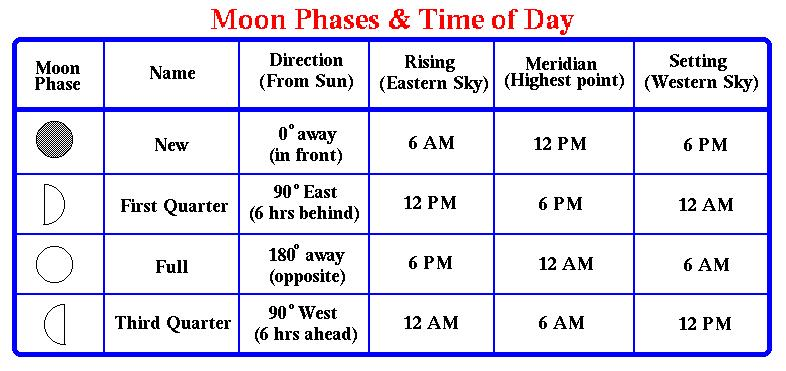
\includegraphics[width=0.7\textwidth]{moon_phases.jpg}
\end{figure}

\subsubsection{Eclipses}
Eclipses occur when the Sun, Moon, and Earth are aligned. A {\bf lunar eclipse} occurs when the Earth lies between the other two, such that the Earth's shadow falls on and blacks out the Moon. A {\bf solar eclipse} occurs when the Moon lies between the Sun and the Earth, so that the Moon block's our view of the Sun (ie. its shadow falls on us).

Since the Moon's orbit is slightly (5 degrees) inclined, eclipses do not happen each month. Eclipses, then, only occur when the Moon passes through the ecliptic; the two locations in which it does are referred to as the {\bf nodes} of its orbit. These times are called {\bf eclipse seasons}, and occur twice per year.

A lunar eclipse occurs when a full moon occurs near a node, a solar eclipse occurs when a new moon occurs near a node.

Since the Moon's shadow has both an {\bf umbra} -- the central area which completely blocks sunlight -- and a {\bf penumbra} -- which only partially blocks sunlight -- these eclipse can look extremely different. If the three objects line up perfectly, we can have a {\bf total lunar eclipse}, in which the Moon is completely blocked during the period of {\bf totality}. More likely is a {\bf partial eclipse}, which only hides a portion of the Moon. Finally, we have {\bf penumbral lunar eclipses}, which shade the Moon but do not completely blot it out.

During totality, the Moon is completely dark for typically less than an hour, save for the red ring around it formed because Earth's atmosphere bends some of the Sun's light toward the Moon (and, to a far lesser extent, due to {\bf gravitational lensing}).

Similarly, we have total and partial solar eclipses based on whether you are within the Moon's umbra or penumbra. When the Moon is too far away for its umbra to even reach the Earth, we see an {\bf annular eclipse}: a ring of sunlight surrounding the Moon when we are directly behind the umbra; otherwise, we see a partial eclipse.

Since the umbra moves across the Earth at a speed of $1,700$ km/h, an eclipse can last no more than a few minutes for any given location on Earth.

The location of the nodes in the Moon's orbit slowly change over time. This gives us an eclipse cycle of 18 years 11.3 days; we call this the {\bf Saros Cycle}. Of course, this only tells us when eclipses will occur, not where they will be visible from on Earth or whether they will be total or partial.

\subsection{Planets}
We can see five planets with the naked eye: Mercury, Venus, Mars, Jupiter, and Saturn. Mercury is rarely visiable, and only near sunrise or sunset. Venus can often be seen shining brightly in the evening (in the West) or before dawn (in the East). Jupiter, when visible, is the brightest star at night. Mars is often recognizeable by its red hue. Saturn has no distinguishing features, but can be identified with star charts.

Planets have different paths of motion that do stars, which is why the word for planet in Greek means ``wandering star''. The planets usually move Eastward through constellations, but sometimes go through periods of {\bf apparent retrograde motion} for anywhere between a few weeks and a few months. This retrograde motion occurs when the Earth ``passes'' the other planet, ie. when their orbits are in line with the Sun.

{\bf Stellar parallax} is the phenomenon of stars appearing to move at different rates given different angles; given the extremely great distances between us and the stars, this is not detectable by the human eye -- though it can be detected by telescopes.


\section{Definitions}
\subsection{Basic Astronomical Objects}
\begin{itemize}
\item a {\bf star} is a large, glowing ball of gas that generates heat and light through nuclear fusion in its core. Our Sun is a star.
\item a {\bf planet} is a moderately large object that orbits a star and shines primarily by reflecting light from its star. According to a definition
approved in 2006, an object can be considered a planet only if it (1) orbits a star; (2) is large enough for its own gravity to make
it round; and (3) has cleared most other objects from its orbital path. An object that meets the first two criteria but has not
cleared its orbital path, like Pluto, is designated a dwarf planet.
\item a {\bf moon (or satellite)} is an object that orbits a planet. The term satellite can refer to any object orbiting another object.
asteroid A relatively small and rocky object that orbits a star.
\item a {\bf comet} is a relatively small and ice-rich object that orbits a star.
\end{itemize}

\subsection{Collections of Astronomical Objects}
\begin{itemize}
\item a {\bf solar system} is the Sun and all the material that orbits it, including the planets, dwarf planets, and small solar system bodies. Although the term solar system technically refers only to our own star system (solar means “of the Sun”), it is often applied to other star systems as well.
\item a {\bf star system} is a star (sometimes more than one star) and any planets and other materials that orbit it.
\item a {\bf galaxy} is a great island of stars in space, containing from a few hundred million to a trillion or more stars, all held together by gravity and
orbiting a common center.
\item a {\bf cluster (or group) of galaxies} is a collection of galaxies bound together by gravity. Small collections (up to a few dozen galaxies)
are generally called groups, while larger collections are called clusters.
\item a {\bf supercluster} is a gigantic region of space where many individual galaxies and many groups and clusters of galaxies are packed more
closely together than elsewhere in the universe.
\item the {\bf universe (or cosmos)} are the sum total of all matter and energy -- that is, all galaxies and everything between them.
observable universe The portion of the entire universe that can be seen from Earth, at least in principle. The observable universe is
probably only a tiny portion of the entire universe.
\end{itemize}

\subsection{Astronomical Distance Units}
\begin{itemize}
\item an {\bf astronomical unit (AU)} is the average distance between Earth and the Sun, which is about 150 million kilometers. More technically,
1 AU is the length of the semimajor axis of Earth’s orbit.
\item a {\bf light-year} is the distance that light can travel in 1 year, which is about 9.46 trillion kilometers.
\end{itemize}

\subsection{Terms Relating to Motion}
\begin{itemize}
\item {\bf rotation} is the spinning of an object around its axis. For example, Earth rotates once each day around its axis, which is an imaginary
line connecting the North Pole to the South Pole.
\item an {\bf orbit (revolution)} is the orbital motion of one object around another. For example, Earth orbits around the Sun once each year.
\item the {\bf expansion (of the universe)} is the increase in the average distance between galaxies as time progresses. Note that while the universe as a whole is expanding, individual galaxies and galaxy clusters do not expand.
\end{itemize}


\section{Formulae and Values}
The {\bf speed of light} is approximately $300,000$ km/h. A {\bf light-year} is the distance light can travel in one year: $9.46 * 10^{12}$ km, or roughly 10 trillion. Note that based on the speed of light, and since the universe formed roughly 14 billion years ago, the distance of 14 billion light-years forms the boundary of the {\bf observable universe}. Note that this does not place a size limit on the entire universe, only on the portion that we can (and will ever be able to) see.

Our solar system was formed 4.5 billion years ago, when about $2\%$ of the galaxy's original Hydrogen and Helium had been converted to heavier elements. Thus the cloud which formed our galaxy was roughly $98\%$ Hydrogen and Helium. The $2\%$ of other materials form the core of the rocky planets in our systems, ie. the Earth.

The {\bf Andromeda galaxy} is roughly 2.5 million light-years away and about $100,000$ light-years in diameter. {\bf Sirius}, the brightest star visible in the night sky, is 8 light-years away. {\bf Alpha Centauri}, the closest star system to our own (a three star system), is 4.4 light-years away.

{\bf Angular size}, physical size, and distance are related as \[ \frac{l_{angular}}{360} = \frac{l_{physical}}{2\pi d} \]

\end{document}
